\smallframetitle

\section{From 17/06/24 to 21/06/24}
\insertsectionframe

\subsection{Road detection method - in progress}
\insertsubsectionframe

\begin{frame}{Methodology}
    We have seen that one classification with either DBScan or HDBScan isn't enough. So, why not combining them.
    \begin{block}{The base idea}
        We will combine the clusters of DBScan, HDBScan and OPTICS (another density base clustering method) to try to find roads.
    \end{block}

    \begin{block}{One problem}
        We are now able to detect road/railways but the problem is that there is still little clusters that are useless.
    \end{block}
\end{frame}

\begin{frame}{New method illustration (1/2)}
    \begin{columns}
        \begin{column}{0.4\paperwidth}
            \begin{figure}
                \boxed{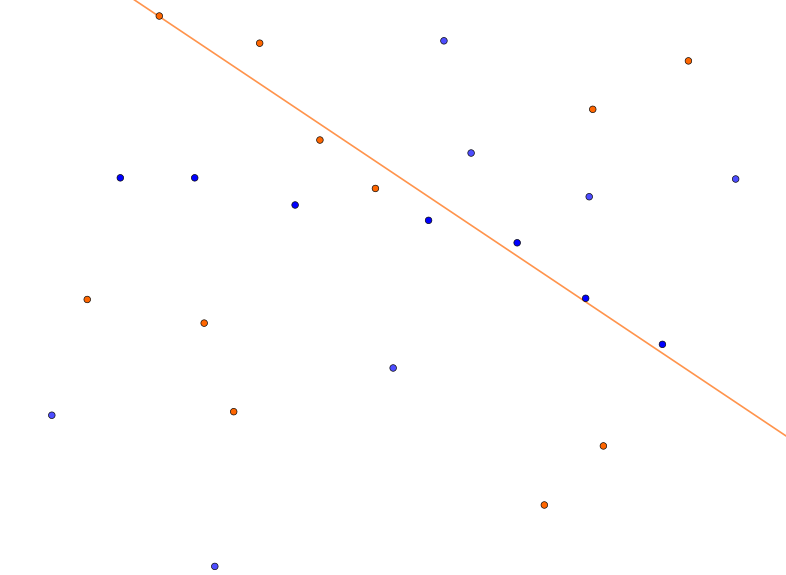
\includegraphics[width=0.4\paperwidth]{images/road_detection/clust1.png}}
                \caption{One clustering method}
            \end{figure}
        \end{column}
        \begin{column}{0.4\paperwidth}
            \begin{figure}
                \boxed{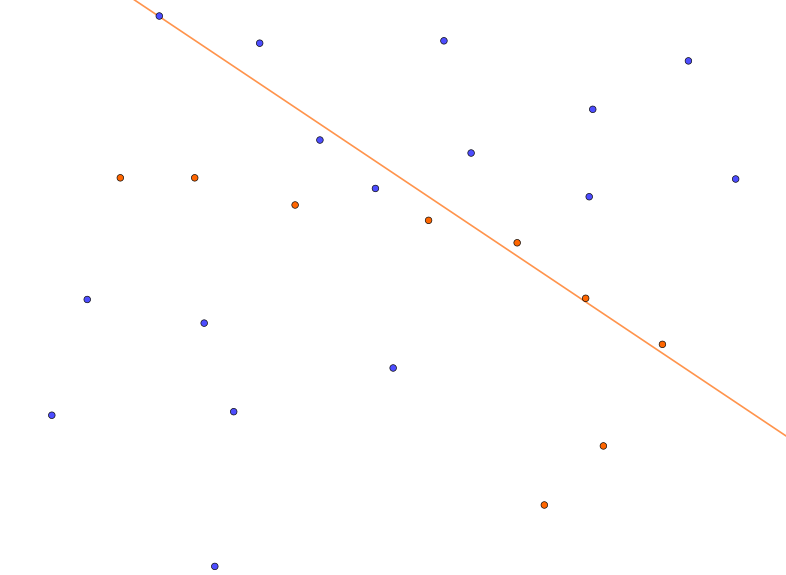
\includegraphics[width=0.4\paperwidth]{images/road_detection/clust2.png}}
                \caption{Another clustering method}
            \end{figure}
        \end{column}
    \end{columns}
\end{frame}

\begin{frame}{New method illustration (2/2)}
    \begin{columns}
        \begin{column}{0.4\paperwidth}
            \begin{figure}
                \boxed{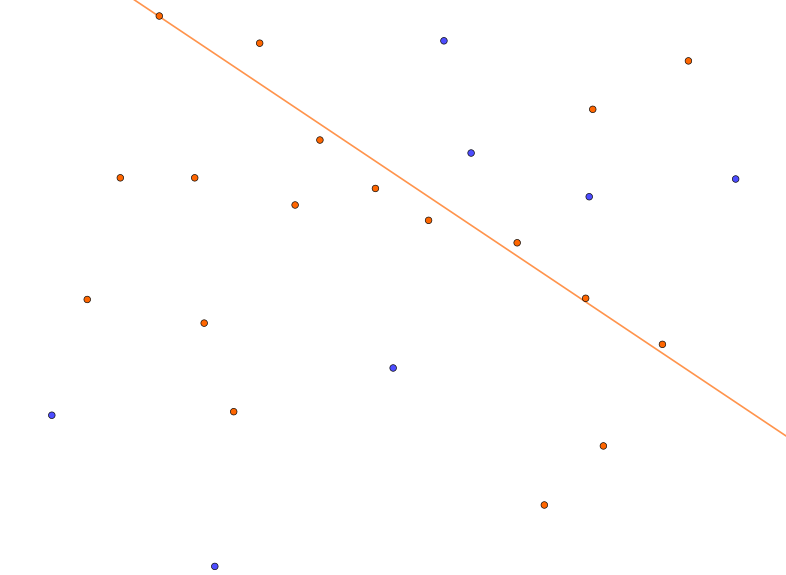
\includegraphics[width=0.4\paperwidth]{images/road_detection/merge_clust.png}}
                \caption{Merge of the clusters}
            \end{figure}
        \end{column}
        \begin{column}{0.4\paperwidth}
            \begin{figure}
                \boxed{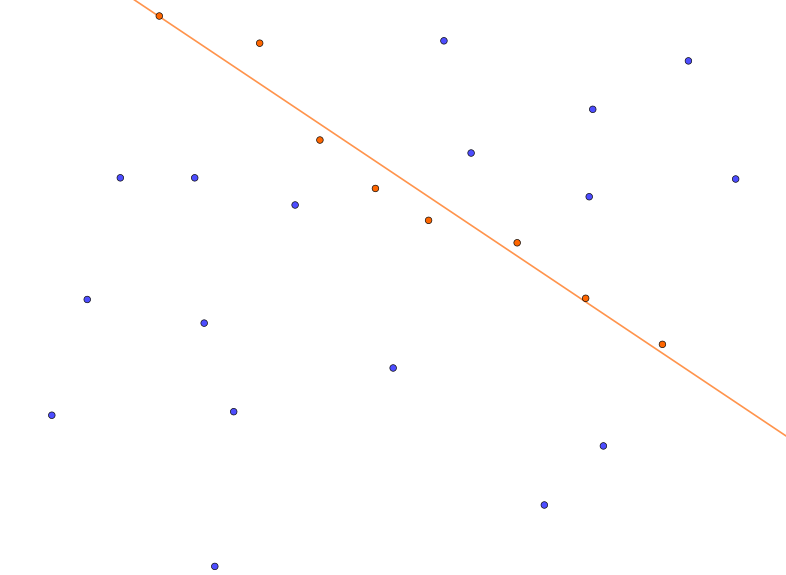
\includegraphics[width=0.4\paperwidth]{images/road_detection/elimination.png}}
                \caption{Elimination of noise}
            \end{figure}
        \end{column}
    \end{columns}
\end{frame}

\begin{frame}{DBScan clustering}
    \begin{figure}
        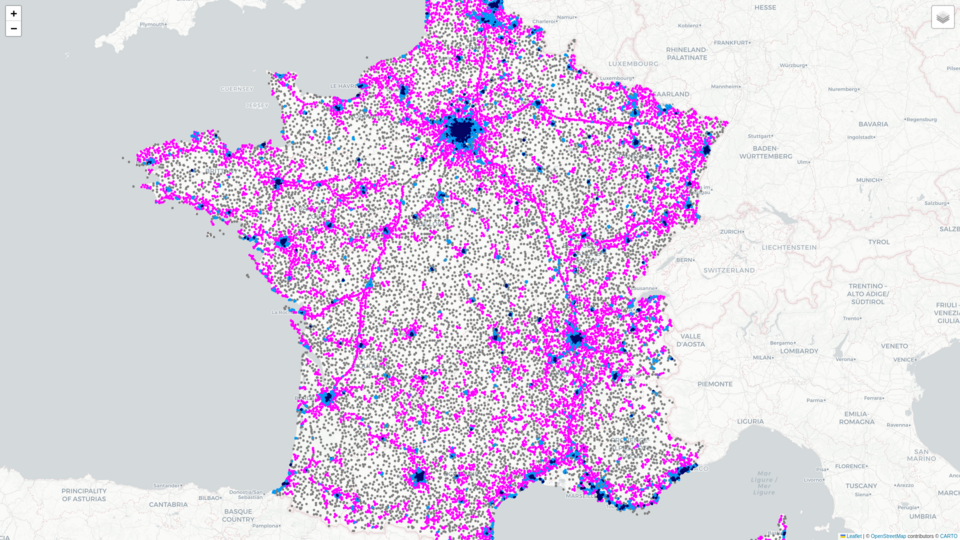
\includegraphics[height=0.6\paperheight]{images/cartes/road_detection/dbs.png}
        \caption{DBScan clustering}
    \end{figure}
\end{frame}

\begin{frame}{HDBScan clustering}
    \begin{figure}
        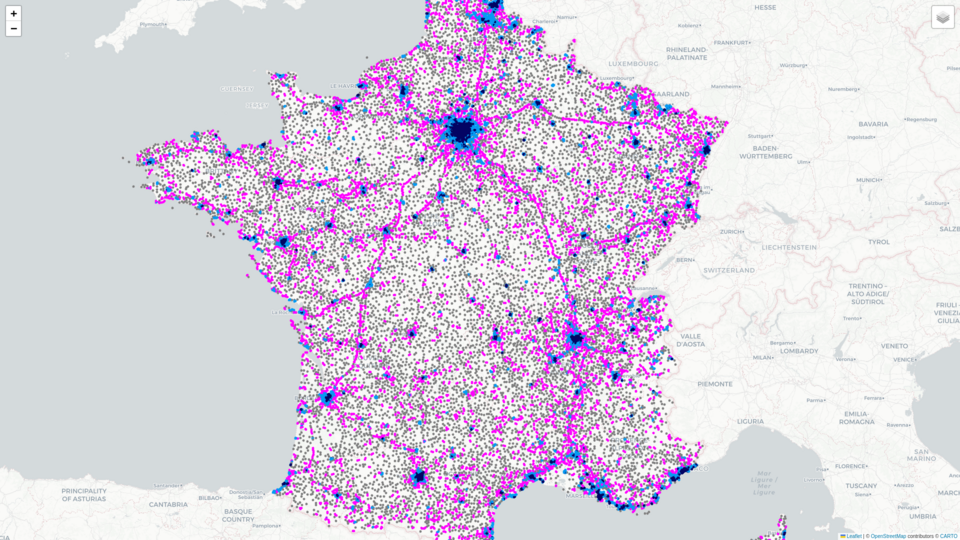
\includegraphics[height=0.6\paperheight]{images/cartes/road_detection/hdb.png}
        \caption{HDBScan clustering}
    \end{figure}
\end{frame}

\begin{frame}{OPTICS clustering}
    \begin{figure}
        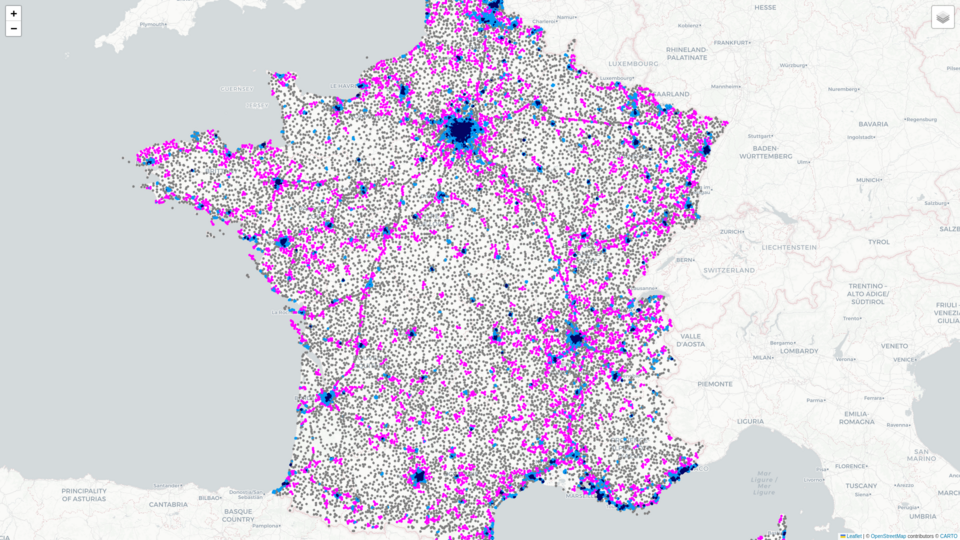
\includegraphics[height=0.6\paperheight]{images/cartes/road_detection/opt.png}
        \caption{OPTICS clustering}
    \end{figure}
\end{frame}

\begin{frame}{Result}
    \begin{figure}
        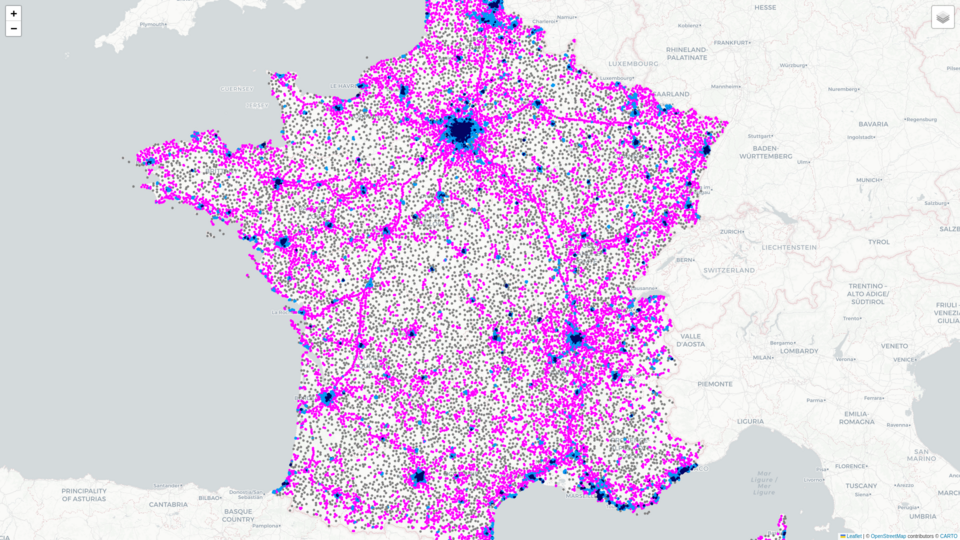
\includegraphics[height=0.6\paperheight]{images/cartes/road_detection/res.png}
        \caption{Road detection}
    \end{figure}
\end{frame}

\subsection{More details and problems}
\insertsubsectionframe

\begin{frame}{Detailed clusters detected}
    \begin{figure}
        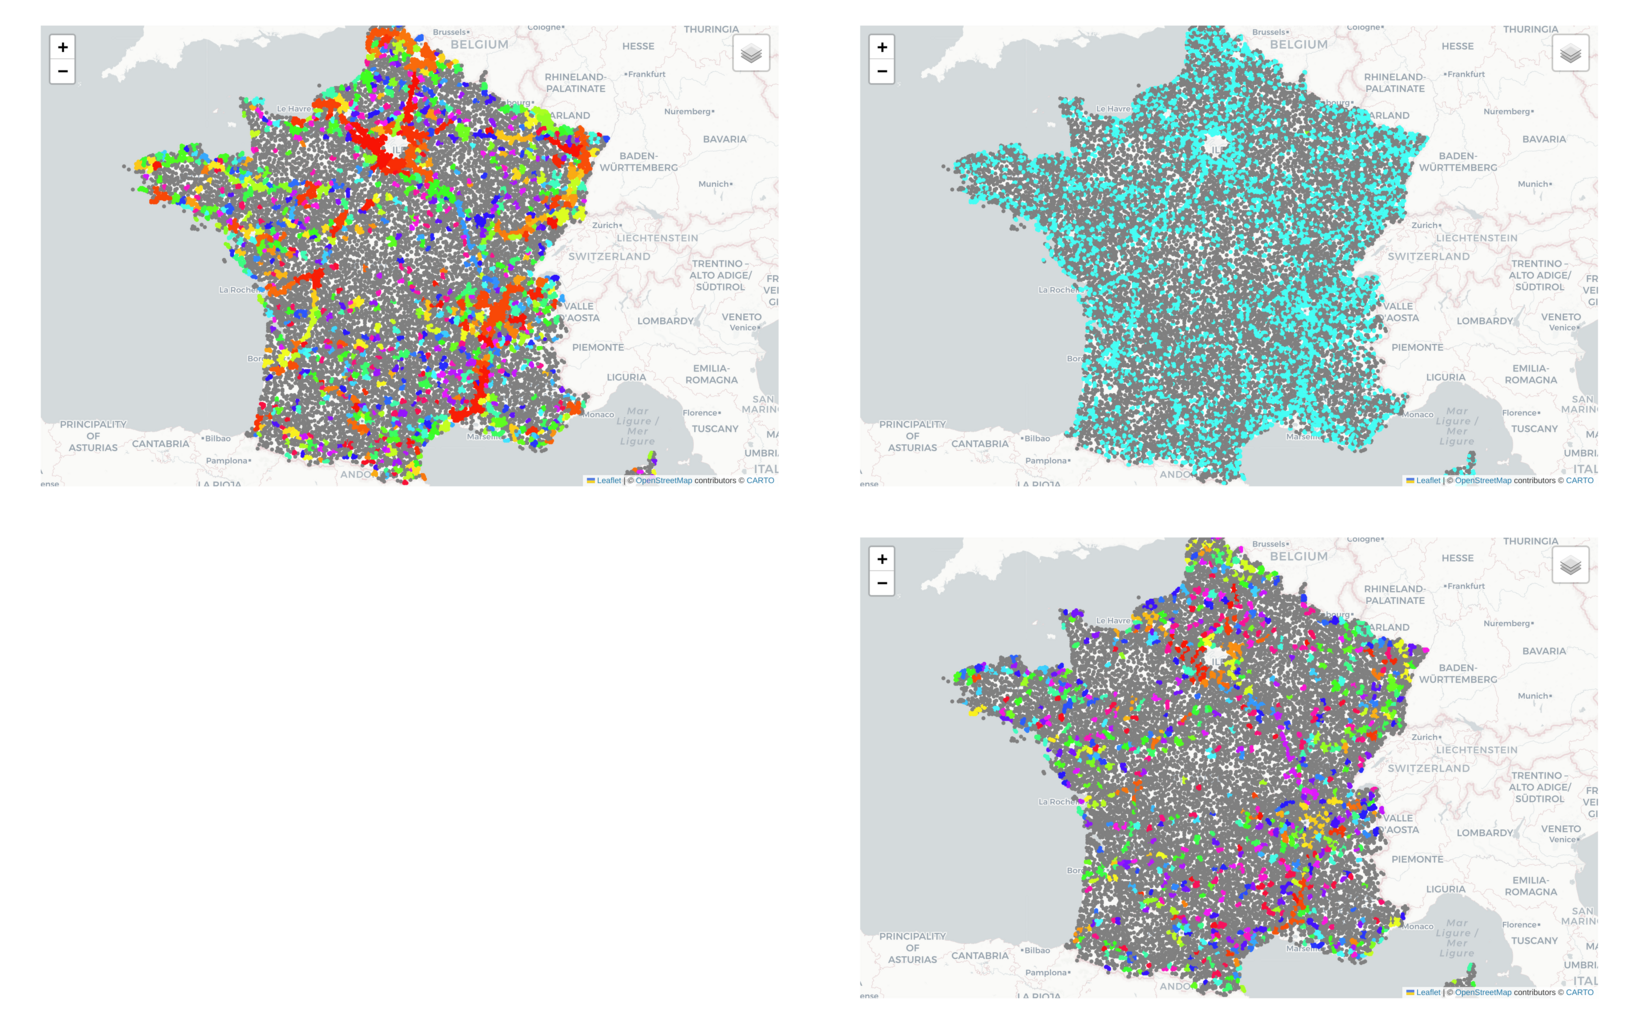
\includegraphics[height=0.6\paperheight]{images/clusters_road_detection.html.png}
        \caption{Detailed clusters detected in coutryside by each method}
    \end{figure}
\end{frame}

\begin{frame}{Problems and ideas}
    \begin{block}{Problems}
        \begin{itemize}
            \item A lot of little citys detected : not only roads ;
            \item The areas around big citys are a mess ;
            \item HDBScan has only one cluster.
        \end{itemize}
    \end{block}

    \begin{block}{Ideas}
        \begin{itemize}
            \item Refine the parameters of each method ;
            \item Use linear regressions to detect parts of roads and maybe help propagate them.
        \end{itemize}
    \end{block}
\end{frame}

\subsection{Altair AI Studio Software Review}
\insertsubsectionframe

\begin{frame}{Altair AI Studio Software Review}
    Objective is to evaluate Altair AI Studio for their potential to enhance our research on classifying the terrain of mobile base stations.
    Available at: \url{https://altair.com/altair-ai-studio}
    \begin{block}{Altair AI Studio}
        This is a platform designed for data analysis and machine learning model building. Possible benefits for us:
        \begin{itemize}
            \item Supports clustering and classification algorithms.
            \item Support for various machine learning algorithms.
            \item Enables effective result visualization (graphs) for enhanced analysis.
        \end{itemize}
    \end{block}
    \begin{columns}
        \begin{column}{0.4\paperwidth}
            \begin{block}{Key Features:}
                \begin{itemize}
                    \item Integration with various data sources.
                    \item Interactive model creation and testing.
                    \item Support for various machine learning algorithms.
                \end{itemize}
            \end{block}
        \end{column}
        \begin{column}{0.4\paperwidth}
            \begin{block}{Users:}
                \begin{itemize}
                    \item Data researchers
                    \item Analysts
                    \item Machine learning developers
                \end{itemize}
            \end{block}
        \end{column}
    \end{columns}
\end{frame}

\begin{frame}{Example of Usage in Altair AI Studio}
    \begin{figure}
        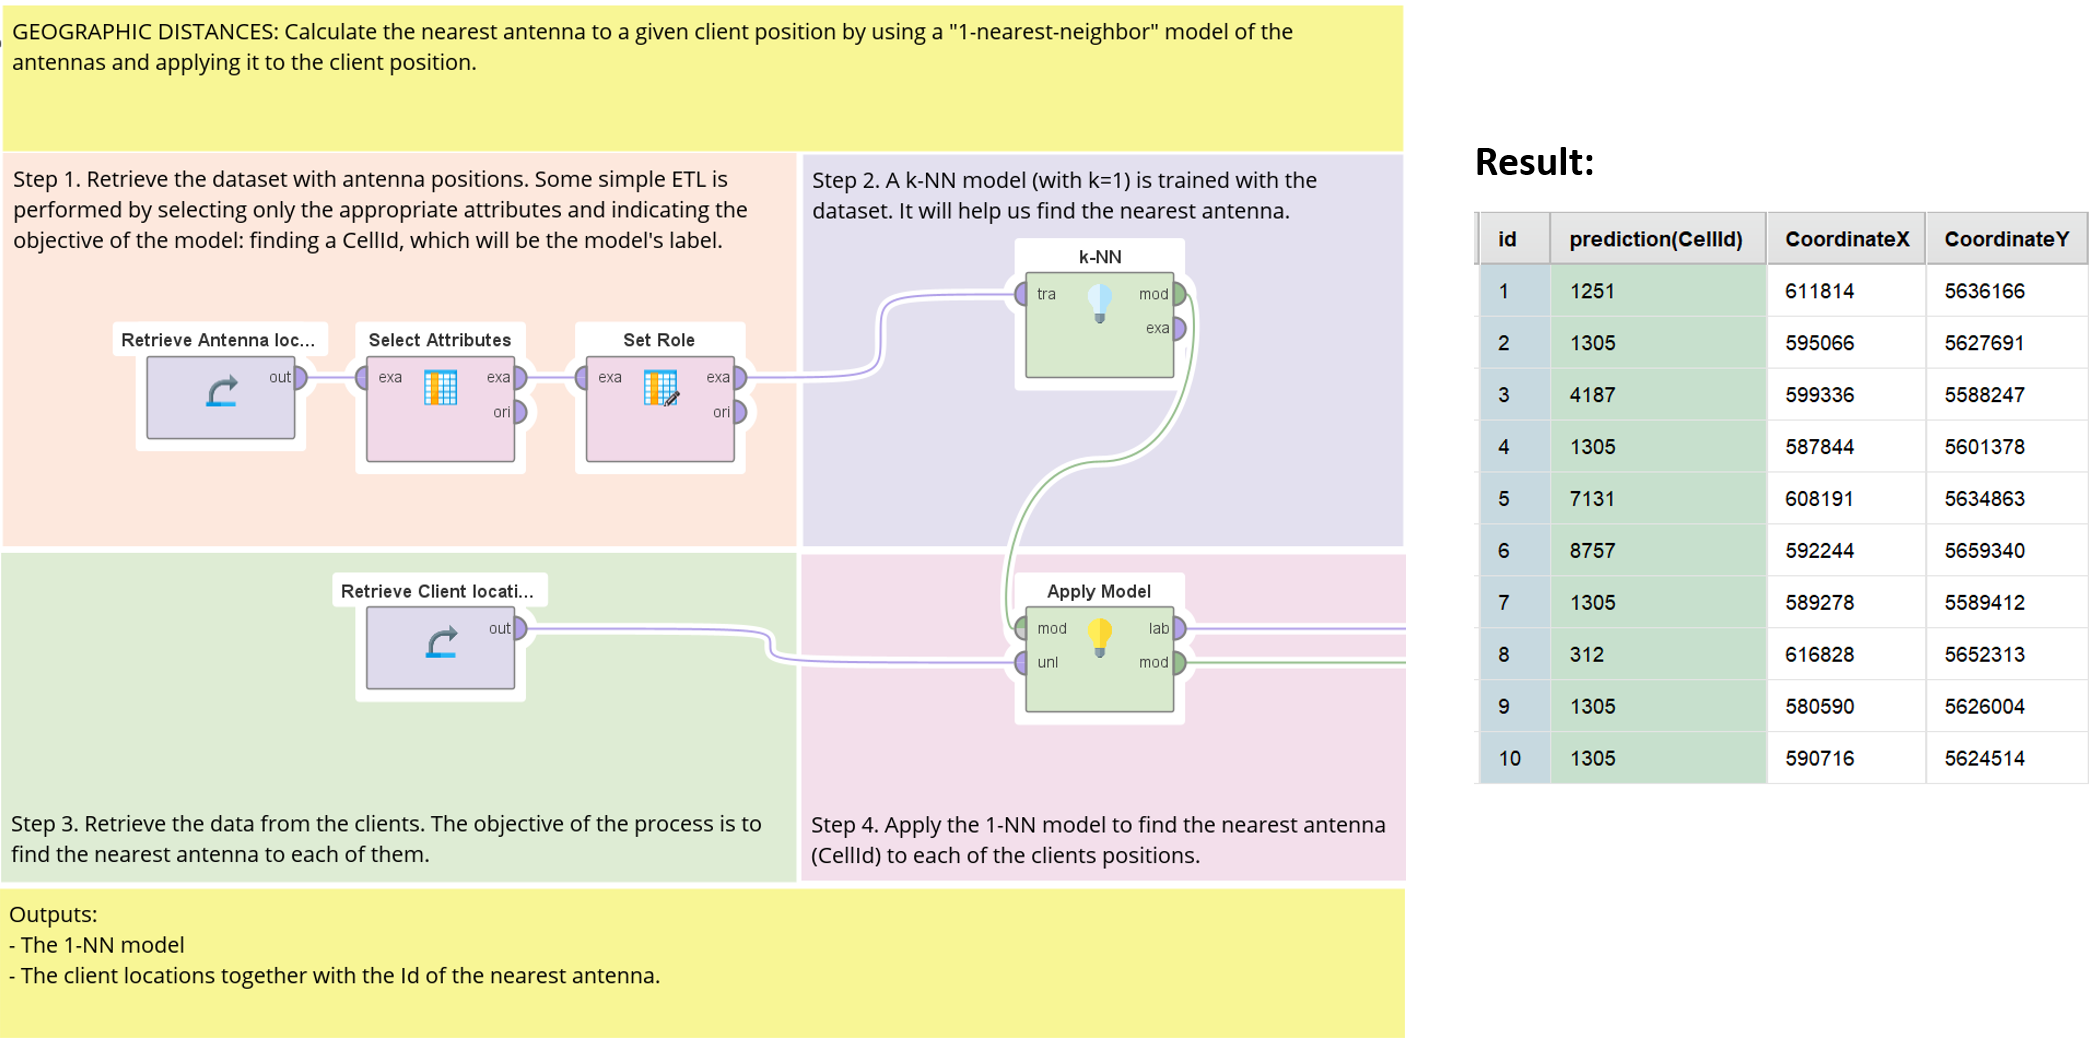
\includegraphics[height=0.6\paperheight]{images/Altair/Altair_proc_exmpl.png}
        \caption{How Altair AI Software works}
    \end{figure}
\end{frame}


\subsection{New Possible Approach for Terrain Classification}
\insertsubsectionframe

\begin{frame}{More accurate verification of the classification of base station locations}
We want to validate and enhance the previous classification of base station locations by leveraging a new geographic dataset. 
We found and will try to use a comprehensive dataset from \url{data.enseignementsup-recherche.gouv.fr}, which includes precise geographic data points across France with pre-defined zone classifications.
\begin{block}{Methodology for Base Station Classification}
    Previously, we worked with a dataset containing locations of all base stations. Now, we utilize an additional dataset with geographic points across France, each classified into zones (urban, suburban, rural). By comparing base station coordinates with these geographic points, we determine the zone of each base station. The closest geographic point's classification is assigned to the base station, providing a more accurate terrain classification.
\end{block}
    \begin{block}{Benefits:}
        \begin{itemize}
            \item Cross-reference base station coordinates with geographic data points to accurately assign zone classifications.
            \item Provides an additional layer of verification and accuracy for our classification methods.
        \end{itemize}
    \end{block}
\end{frame}



\begin{frame}{Classification of points in the new dataset}
    \begin{figure}
        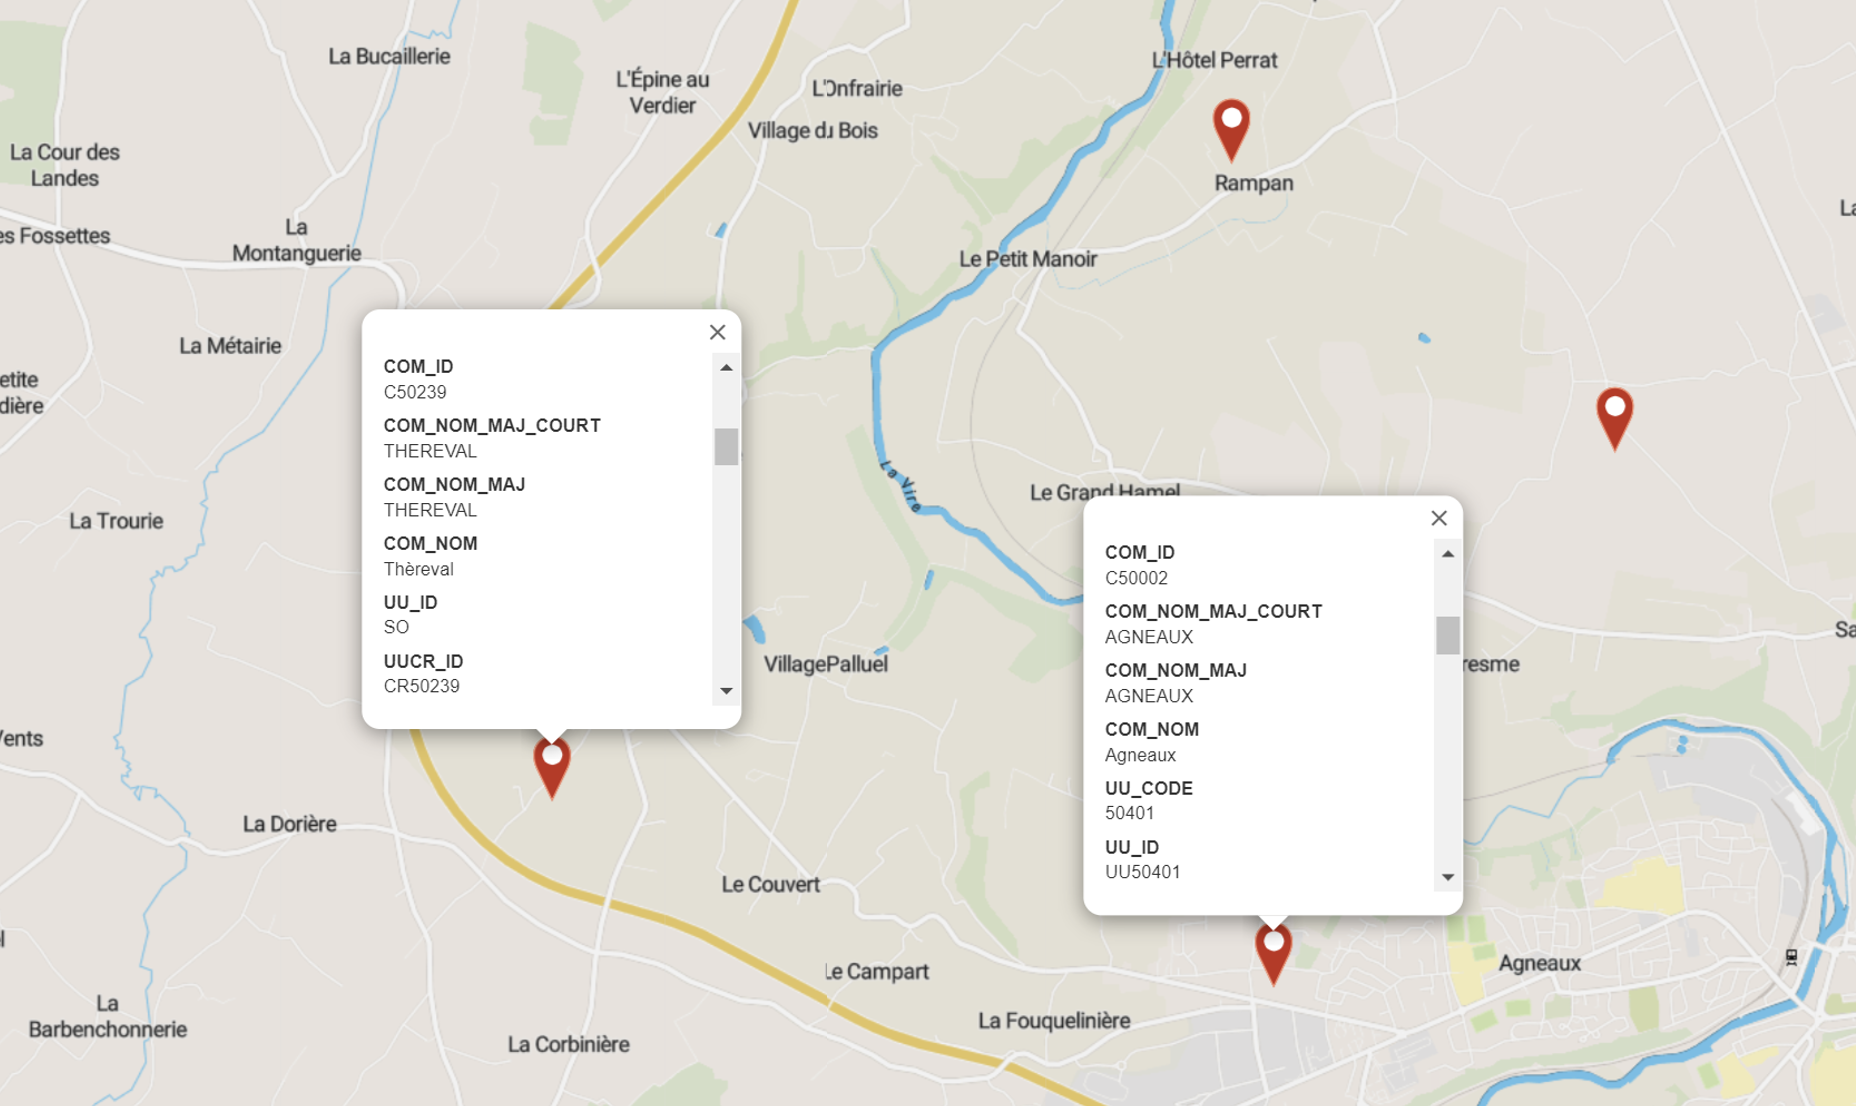
\includegraphics[height=0.6\paperheight]{images/Geo_approach/New_dataset_points_ill.png}
        \caption{Classification of points from the new dataset}
    \end{figure}
\end{frame}
\begin{frame}{Classification of points in the new dataset}
    \begin{block}{Geographic identifiers:}
        \begin{itemize}
        \item UU (Urban Units): Areas classified as urban units.
        \item CR (Rural Communes): Areas classified as rural communes.
        \item AU (Urban Areas): Larger urban areas or agglomerations.
        \end{itemize}
    \end{block}
    \begin{block}{Methodology and Challenges}
            This method helps classify base station locations by comparing them with geographic data points. However, we need to preprocess the dataset carefully and address the issue of having a limited number of points. To ensure high accuracy, we might need to augment the data or combine it with other datasets for better coverage and precision
    \end{block}
\end{frame}

\subsection{Another new database}
\insertsubsectionframe

\begin{frame}{New possibilities on city/countryside classification}
    \begin{columns}
        \begin{column}{0.4\paperwidth}
            \begin{figure}
                \boxed{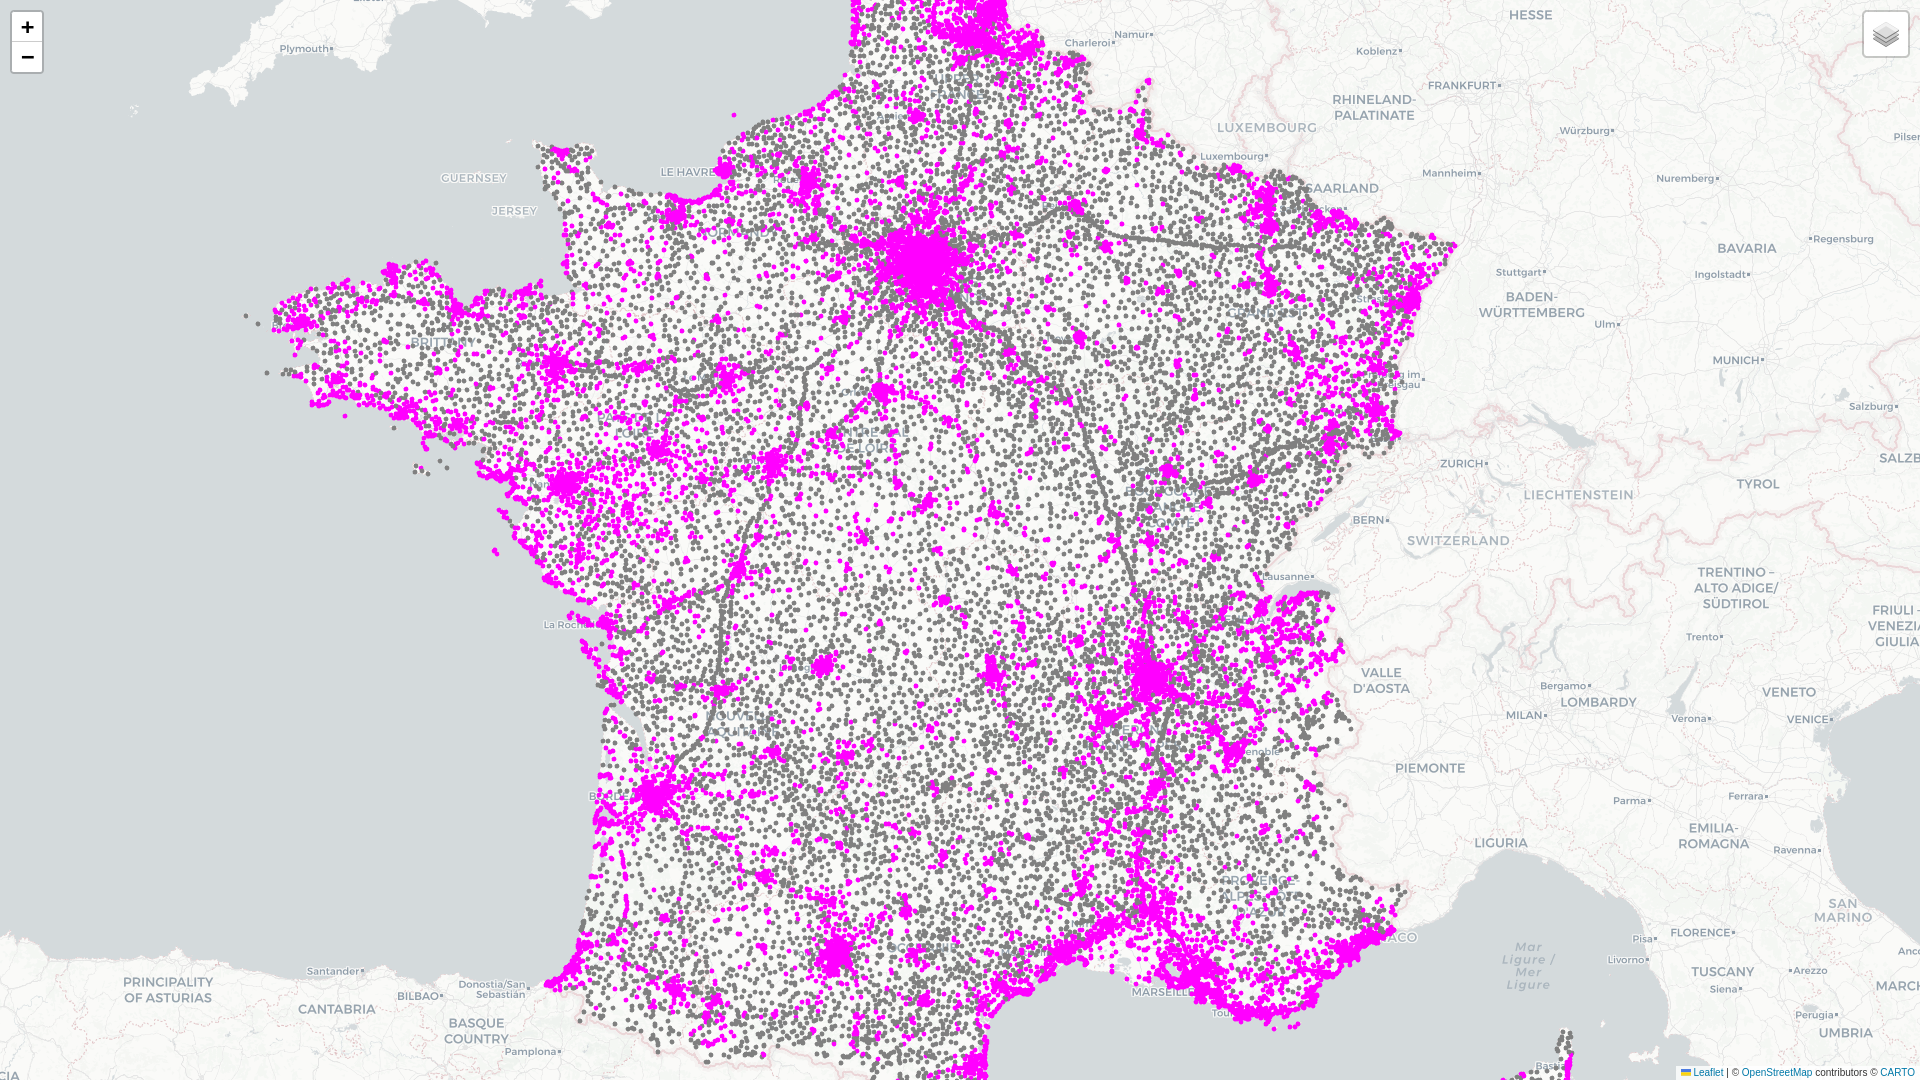
\includegraphics[width=0.4\paperwidth]{images/cartes/new_databases/new_database.png}}
                \caption{Database we presented last week}
            \end{figure}
        \end{column}
        \begin{column}{0.4\paperwidth}
            \begin{figure}
                \boxed{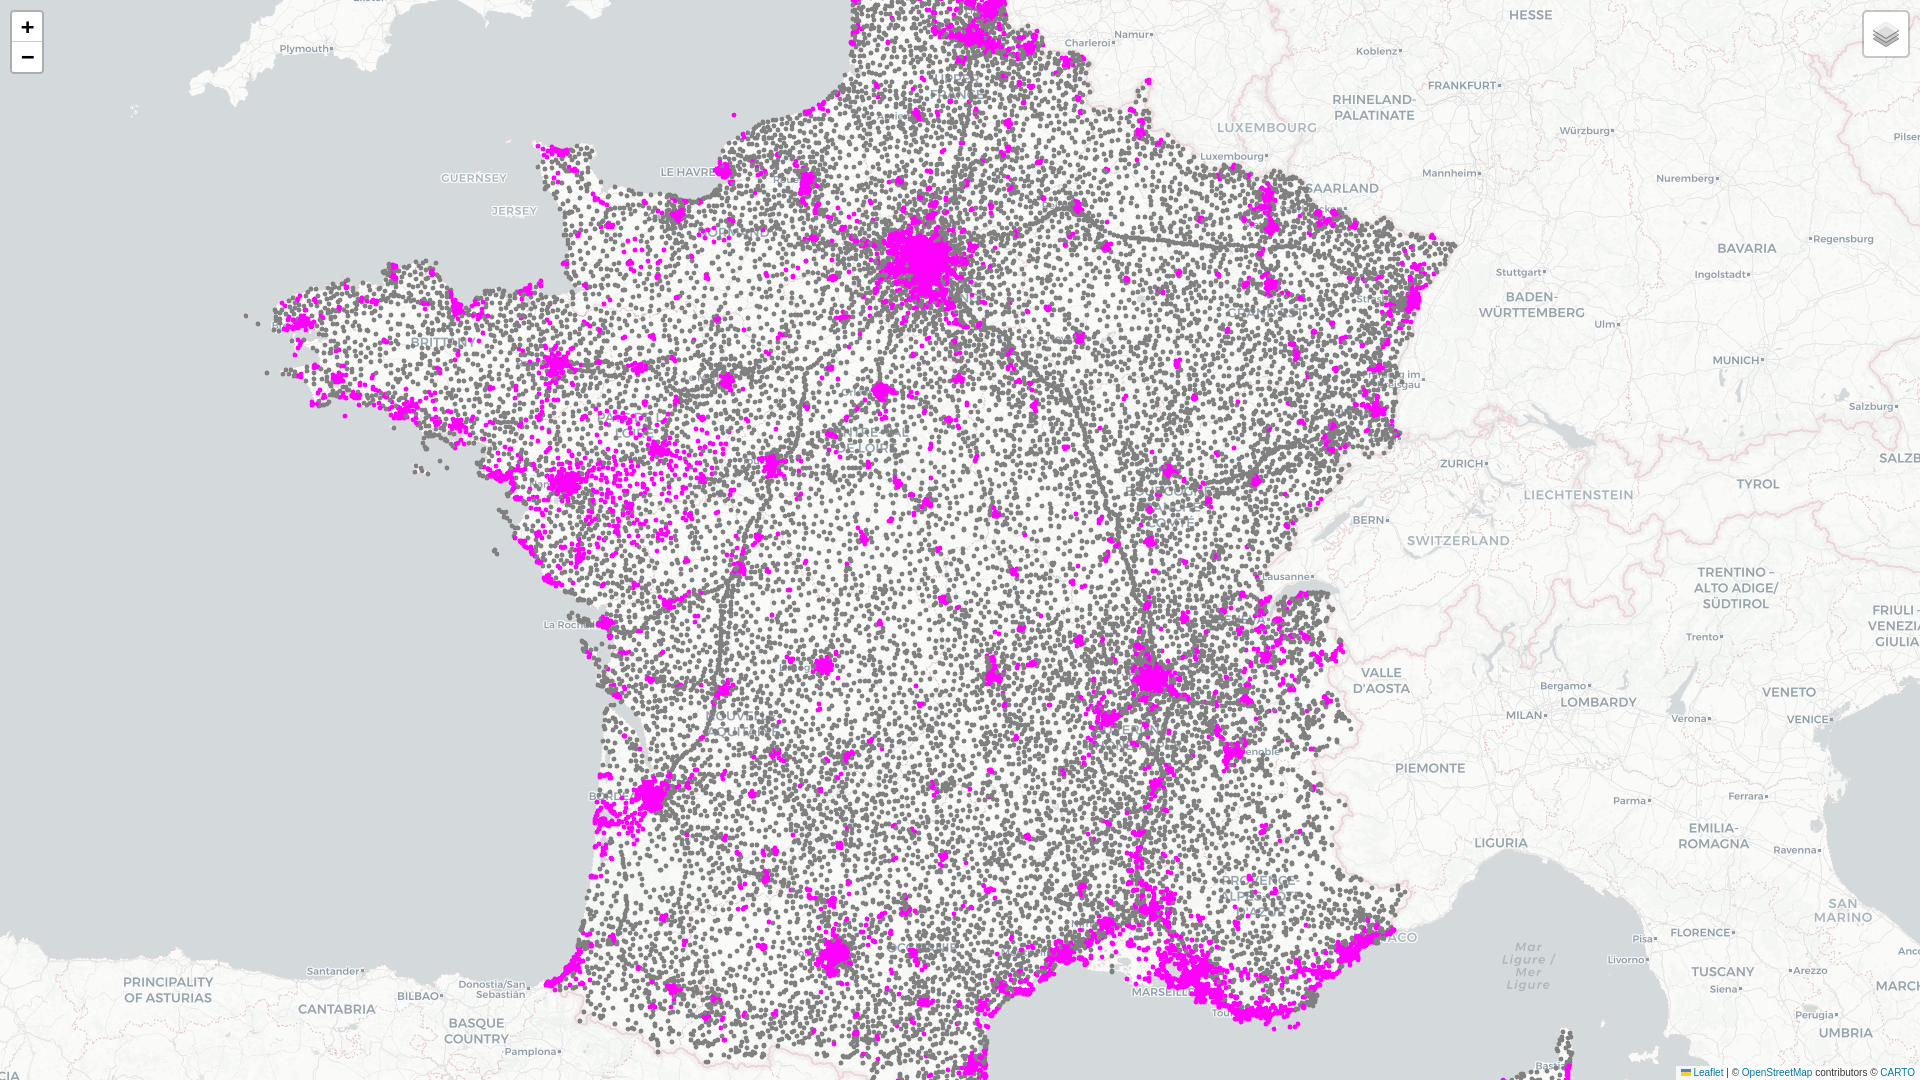
\includegraphics[width=0.4\paperwidth]{images/cartes/new_databases/new-new_database.png}}
                \caption{A new database}
            \end{figure}
        \end{column}
    \end{columns}
\end{frame}

\begin{frame}{What's this?}
    We found a new database on the population of each french commune in 2021\footnote{\url{https://www.insee.fr/fr/statistiques/7739582}}.
    \begin{block}{INSEE?}
        It is the National Institute of Statistics and Economics Studies. It collects, analyses and disseminates information on the French economy and society.
    \end{block}

    \begin{block}{Why this one?}
        Firstly, this database is really recent (updated on 26/01/2024). Then, the other database we introduced was to permisive in the definition of what is a city (a commune with more than $2000$ inhabitants).
        So we wanted something more flexible.
    \end{block}
\end{frame}

\subsection{Back to road detection}
\insertsubsectionframe

\begin{frame}{HDBScan parameters adaptation}
    \begin{figure}
        \boxed{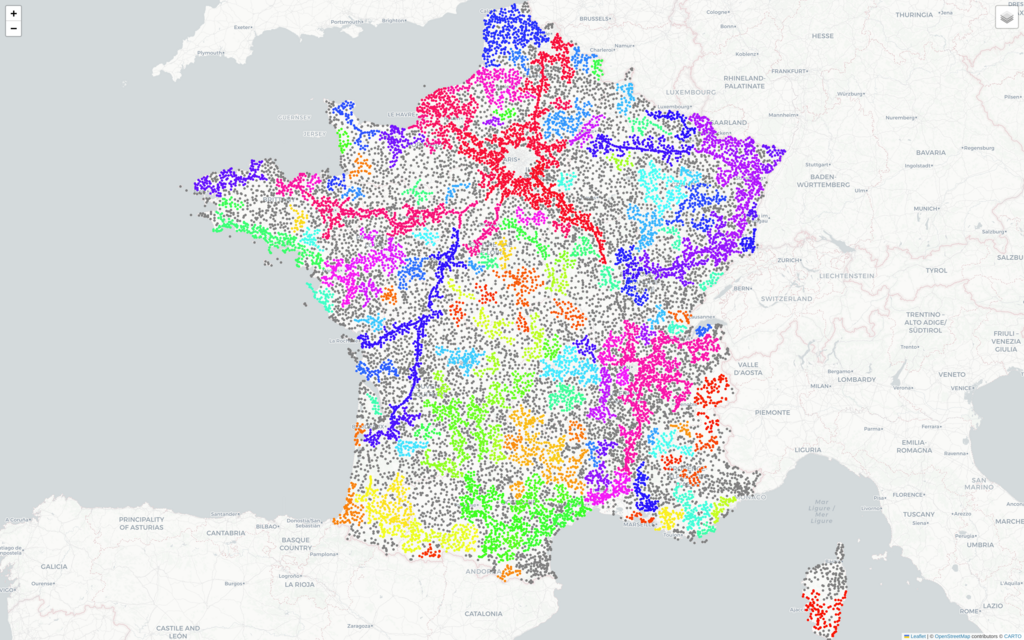
\includegraphics[height=0.6\paperheight]{images/hdbscan_roads_crude.png}}
        \caption{Result of HDBScan with new parameters on countryside to detect roads}
    \end{figure}
\end{frame}

\begin{frame}{A bit of math theory (1/2)}
    \begin{block}{Multiple linear regression}
        Let a dataset be composed of $m$ vectors$\ensuremath{\left(x^{i}\right)_{i\in\left\{ 1...m\right\} }}$
        of $\mathbb{R}^{n}$, ie $\forall i\in\{1,...,m\}$, $x^{i}=(x_{1}^{i},\dots,x_{n}^{i})$. 

        Let $\ensuremath{\left(y^{i}\right)_{i\in\left\{ 1...m\right\} }}$
        be $m$ associated values in $\mathbb{R}$.

        Then, we can find a linear function $f:\mathbb{R}^{n}\rightarrow\mathbb{R}$
        (ie $f(x_{1},\dots,x_{n})=c_{1}x_{1}+\dots+c_{n}x_{n}$) that minimises
        the error : $\begin{Vmatrix}\sum_{i=1}^{m}(f(x^{i})-y^{i})\end{Vmatrix}$

        $f$ is called a multiple linear regression associated to $\ensuremath{\left(x^{i}\right)_{i\in\left\{ 1...m\right\} }}$
        and $\ensuremath{\left(y^{i}\right)_{i\in\left\{ 1...m\right\} }}$.
    \end{block}
    \begin{figure}
        \boxed{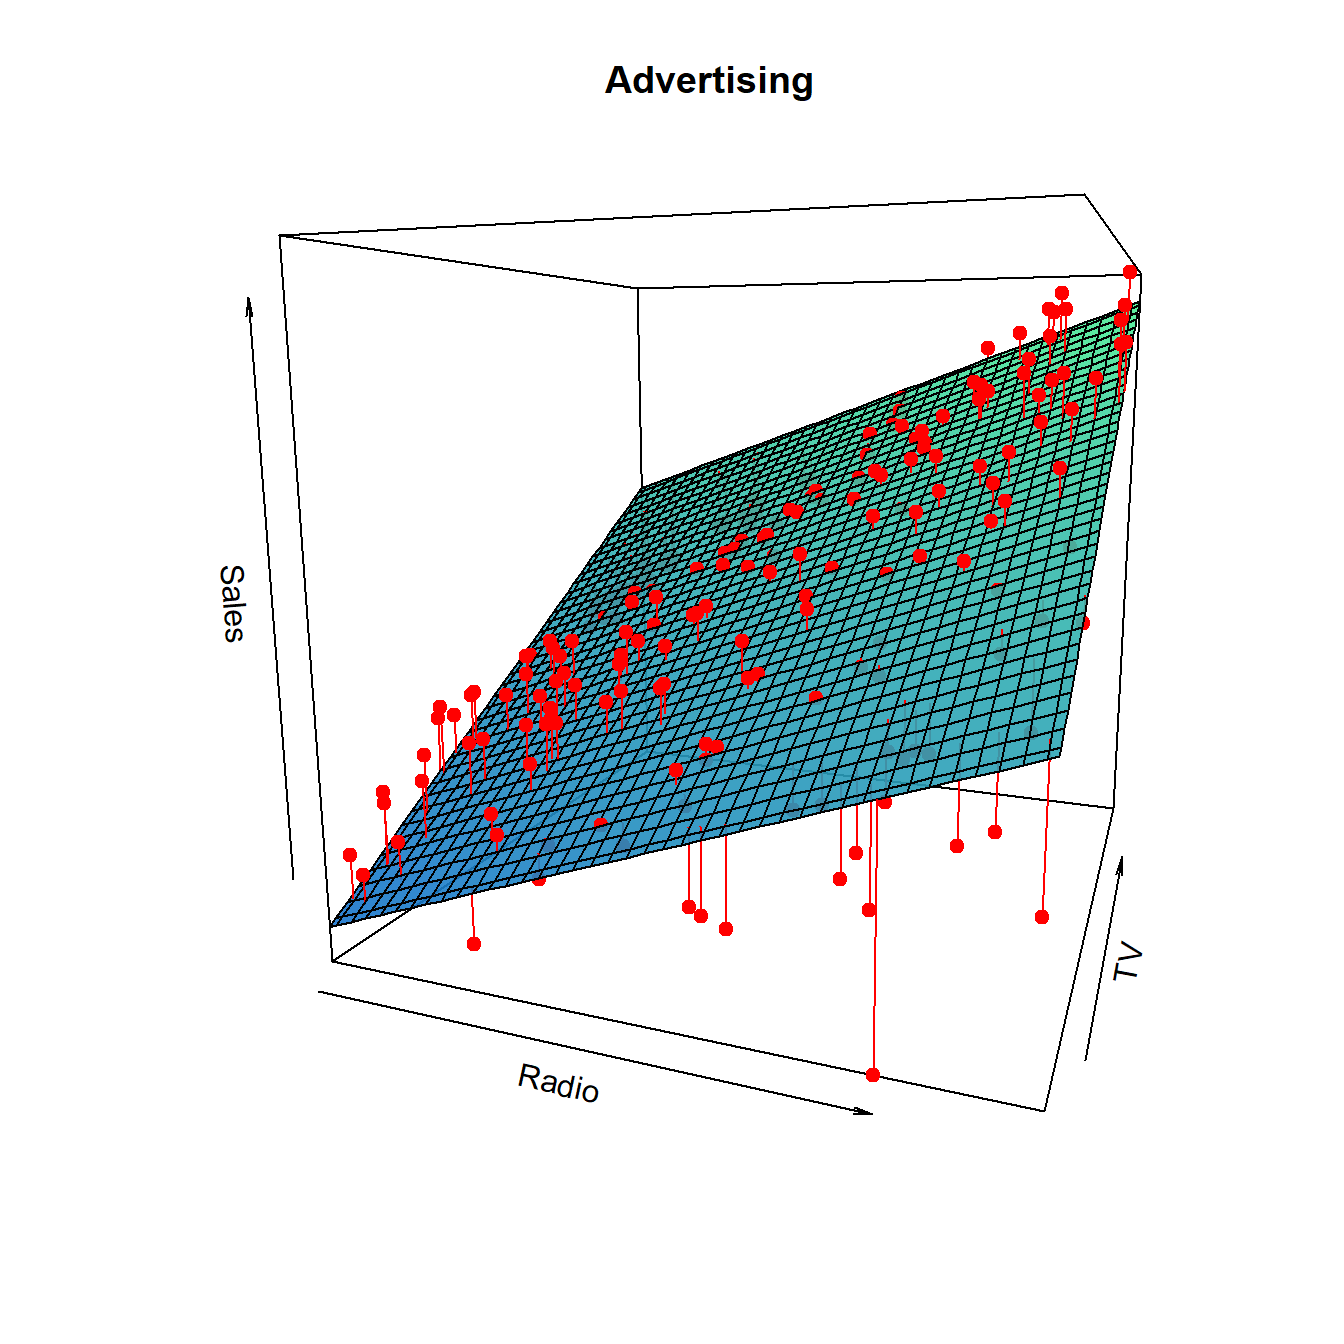
\includegraphics[height=0.3\paperheight]{images/multiple_linear_regression.png}}
        \caption{Example of multiple linear regression with $n=2$}
    \end{figure}
\end{frame}

\begin{frame}{A bit of math theory (2/2)}
    \begin{block}{Polynomial regression}
        Let a dataset be composed of $m$ values $\ensuremath{\left(x^{i}\right)_{i\in\left\{ 1...m\right\} }}$ of $\mathbb{R}$. 

        Let $\ensuremath{\left(y^{i}\right)_{i\in\left\{ 1...m\right\}}}$ be $m$ associated values in $\mathbb{R}$.

        We can transform the data in $m$ vectors$\ensuremath{\left(x^{i}\right)_{i\in\left\{ 1...m\right\}}}$
        of $\mathbb{R}^{n+1}$ defined by $(x_{0}^{i},x_{1}^{i},x_{2}^{i},\dots,x_{n}^{i})=(1,x^{i},(x^{i})^{2},\dots,(x^{i})^{n})$, 
        and then apply the multiple linear regression seen earlier on this transormed data.
        
        We therefore obtain a function 
        \[
            f:\begin{cases}
            \mathbb{R}\rightarrow\mathbb{R}\\
            x\mapsto c_{1}+c_{2}x+\dots+c_{n}x^{n}
            \end{cases}
        \]
        
        That is a degree n polynome that approximates the relation between $x$ and $y$.
    \end{block}

    \begin{block}{Quantify the quality of the approximation}
        As for the simple linear regression, we obtain a R coefficient between 0 and 1 that indicates if the approximation is close to the original data 
        (ie if the polynome we find at the end is close to the real appearance of the data).
    \end{block}
\end{frame}

\begin{frame}{Application of the method on each cluster of hdbscan}
    \begin{figure}
        \boxed{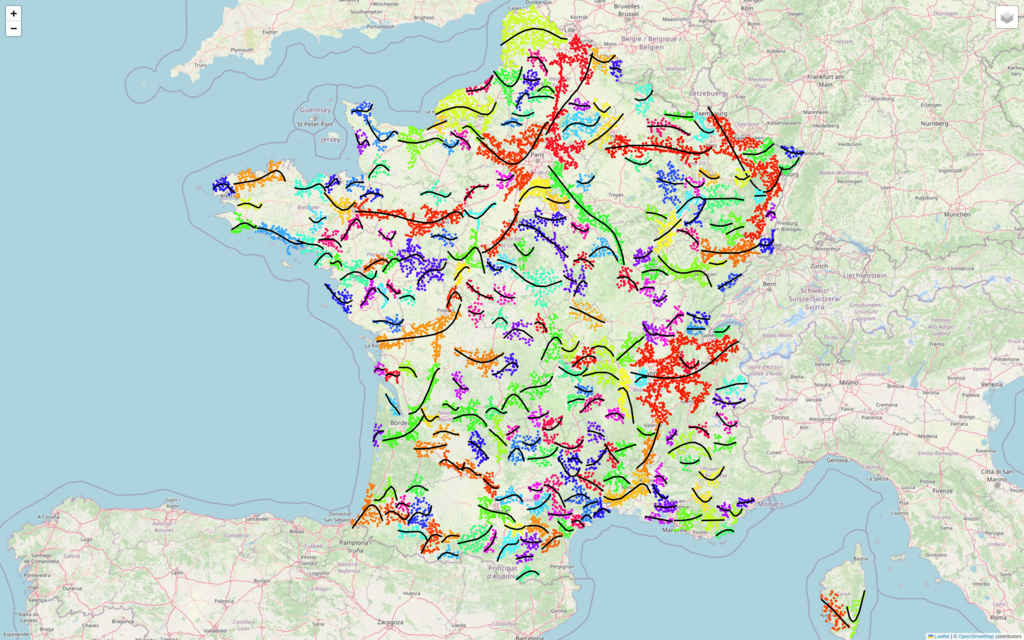
\includegraphics[height=0.6\paperheight]{images/hdbscan_roads.png}}
        \caption{Approximation of each cluster by a degree 20 polynome}
    \end{figure}
\end{frame}

\begin{frame}{Filtration of the cluster by keeping the ones that have a $R$ coefficient above a value}
    \begin{figure}
        \boxed{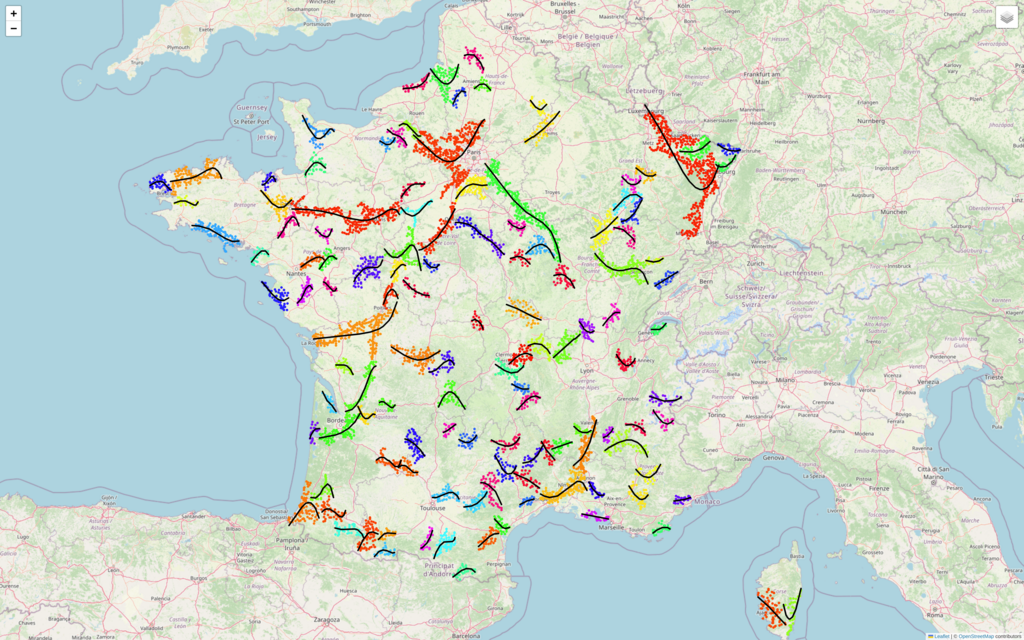
\includegraphics[height=0.6\paperheight]{images/hdbscan_roads_filtered.png}}
        \caption{Approximation of each cluster by a degree 20 polynome, keeping only the ones with a $R$ coefficient above 0.2}
    \end{figure}
\end{frame}